\documentclass[11pt]{amsart}
\usepackage{geometry}                % See geometry.pdf to learn the layout options. There are lots.
\geometry{letterpaper}                   % ... or a4paper or a5paper or ... 
%\geometry{landscape}                % Activate for for rotated page geometry
\usepackage[parfill]{parskip}    % Activate to begin paragraphs with an empty line rather than an indent
\usepackage{graphicx}
\usepackage{amssymb}
\usepackage[all]{xy}
\usepackage{epstopdf}
\usepackage{pdfpages}
\usepackage{hyperref}
\DeclareGraphicsRule{.tif}{png}{.png}{`convert #1 `dirname #1`/`basename #1 .tif`.png}


% these packages make it easy to include figures in the text. 
\usepackage{float}
\restylefloat{figure}

\newcommand{\cX}{\mathcal{X}}
\newcommand{\cC}{\mathcal{C}}
\newcommand{\cF}{\mathcal{F}}
\newcommand{\prox}{\mathrm{prox}}



\begin{document}
{\Large Name: Philip Pham}  \\
\begin{center}
\Large AMATH 515 \hskip 2in Homework Set 2\\
\end{center}

\begin{enumerate}



\item Recall that 
\[
\begin{aligned}
\mbox{prox}_{t f}(y) &= \arg\min_{x} \frac{1}{2t}\|x-y\|^2 + f(x)\\
f_t(y) &= \min_x \frac{1}{2t}\|x-y\|^2 + f(x).
\end{aligned}
\] 
Suppose $f$ is convex. 
\begin{enumerate}
%\item Prove $\mbox{prox}_f(x) + \mbox{prox}_{f^*}(x) = x$.

\item Prove that $f_t$ is convex.
  \begin{proof}
    Let $h(x, y) = \frac{1}{2t}\|x-y\|^2 + f(x)$, so $f_t(y) = \min_x h(x,
    y)$. $h$ is a convex function of $x$ as it is the sum of a $\ell_2$-norm and
    a convex function. Only the first term depends on $y$, which is a
    $\ell_2$-norm, which is convex, so $h$ is convex as a function of $y$.

    Now, using the convexity, we have that
    \begin{align*}
      f_t\left(\lambda y_1 + (1-\lambda)y_2\right)
      &= \min_x h\left(x, \lambda y_1 + (1-\lambda)y_2\right) \\
      &\leq h\left(\lambda x_1 + (1-\lambda)x_2, \lambda y_1 + (1-\lambda)y_2\right) \\
      &\leq \lambda h\left(x_1, y_1\right) + (1-\lambda)h\left(x_2, y_2\right).
    \end{align*}
    We can choose $x_1$ and $x_2$ to be anything. For instance, we could choose
    $x_1 = \arg\min_{x} h\left(x, y_1\right)$ and
    $x_2 = \arg\min_{x} h\left(x, y_2\right)$. In this case, we'd have that
    \begin{align*}
      f_t\left(\lambda y_1 + (1-\lambda)y_2\right)
      &\leq \lambda h\left(x_1, y_1\right) + (1-\lambda)h\left(x_2, y_2\right)
        = \lambda f_t\left(y_1\right) + \left(1 - \lambda\right) f_t\left(y_2\right),
    \end{align*}
    so $f_t$ is convex.
  \end{proof}
  
\item Prove that $\prox_{t f}$ is a single-valued mapping. 
  \begin{proof}
    In $h$, the first term is strongly convex with $\alpha = t^{-1} \gneq
    0$. Since $h$ is the sum of convex functions, $h$ will also be strongly
    convex with $\alpha \gneq 0$. Therefore, $h$ has a unique global minimizer,
    so $\prox_{t f}$ is a single-valued mapping.
  \end{proof}

\item Compute $\prox_{t f}$ and $f_t$, where $f(x) = \|x\|_1$. 
%One way to do this is to consider the scalar case, and explicitly compute $f'(t)$ 
%\[
%f'_t(x) = \frac{1}{t} (x-\prox_{t f}(x)).
%\]
%Now, just find a function that has this derivative. 

  \begin{proof}
    We can rewrite the objective as a sum of positive terms
    \begin{align*}
      \frac{1}{2t}\|x-y\|^2 + \|x\|_1
      &= \sum_{i=1}^n\left[
        \frac{1}{2t}\left(x_i - y_i\right)^2
        +
        |x_i|
        \right].
    \end{align*}
    Each term is independent of each other, so we can minimize each term
    separately. The derivative of each term is undefined at $x_i = 0$, but
    otherwise,
    \begin{equation*}
      \frac{\partial}{\partial x_i}\left(
        \frac{1}{2t}\left(x_i - y_i\right)^2 + |x_i|
      \right)
      = \frac{x_i - y_i}{t} + \operatorname{sign}\left(x_i\right).
    \end{equation*}

    Solving for $x_i$ when $|y_i| \geq t$, we find
    $x_i = y_i - \operatorname{sign}\left(y_i\right)t$. Otherwise, we note that
    the derivative is negative when $x_i < 0$ and positive when $x_i > 0$, so
    the solution must be $x_i = 0$. Thus, we have that
    \begin{equation*}
      \left[\prox_{t f}(y)\right]_i = \begin{cases}
        y_i - \operatorname{sign}\left(y_i\right)t, & |y_i| \geq t; \\
        0, & \text{otherwise.}
      \end{cases}
    \end{equation*}
  \end{proof}

\item Compute $\prox_{t f}$ and $f_t$ for $f = \delta_{\mathbb{B}_{\infty}}(x)$, 
  where $\mathbb{B}_\infty = [-1,1]^n$.

  \begin{proof}
    We can use a similar strategy as the previous problem and treat each term
    separately. In this case, we have that
    \begin{equation*}
      \frac{1}{2t}\|x-y\|^2 + \delta_{\mathbb{B}_{\infty}}(x)
      = \sum_{i=1}^n\left[
        \frac{1}{2t}\left(x_i - y_i\right)^2
        +
        \delta_{[-1,1]}(x_i)
        \right].
      \end{equation*}

      For each term, we have that
      \begin{equation*}
        \frac{1}{2t}\left(x_i - y_i\right)^2 + \delta_{[-1,1]}(x_i) = \begin{cases}
          \frac{1}{2t}\left(x_i - y_i\right)^2, &x_i \in [-1, 1]; \\
          \infty, &\text{otherwise}.
        \end{cases}
      \end{equation*}
      This can easily be seen to be minimized by $x_i = y_i$ when
      $y_i \in [-1, 1]$, $x_i = 1$ when $y_i > 1$ and $x_i = -1$, when
      $y_i < -1$, so we have that
      \begin{equation*}
        \left[\prox_{t f}(y)\right]_i = \begin{cases}
          y_i, & y_i \in [-1, 1]; \\
          -1, & y_i < -1; \\
          1, & y_i > 1.
        \end{cases}
      \end{equation*}      
    \end{proof}
\end{enumerate}

\item More prox identities. 
\begin{enumerate}
%\item Prove $\mbox{prox}_f(x) + \mbox{prox}_{f^*}(x) = x$.

\item Suppose $f$ is convex and let $g(x) = f(x) + \frac{1}{2}\|x-x_0\|^2$. 
  Find formulas for $\prox_{t g}$ and $g_t$ in terms of $\prox_{t f}$ and $f_t$.

  \begin{proof}
    We would like to minimize the objective
    \begin{align*}
      \frac{1}{2t}\|x-y\|^2 + f(x) + \frac{1}{2}\|x-x_0\|^2
      &= \frac{1}{2t}\|x-y\|^2 + \frac{1}{2}\left\|x\right\|^2 + f(x) -
        \left\langle x_0, x \right\rangle + \frac{1}{2}\|x_0\|^2.
    \end{align*}
    We can drop the last term when calculating $\prox_{t g}(y)$ since it does
    not depend on $x$. We have that
    \begin{align*}
      \prox_{t g}(y)
      &= \arg\min_x \frac{1}{2t}\|x-y\|^2 + \frac{1}{2}\|x\|^2 + f(x)        
        - \left\langle x_0, x \right\rangle.
    \end{align*}

    From Problem (2)(c), we'll have that
    \begin{align*}
      \prox_{\frac{t}{2}\| \cdot \|^2}(y) = \frac{1}{1 + t}y.
    \end{align*}

    $x \mapsto -\left\langle x_0, x \right\rangle$ is differentiable, so we can
    differentiate
    $x \mapsto \frac{1}{2t}\|x-y\|^2 -\left\langle x_0, x \right\rangle$, set it
    equal to $0$, and solve for $x$ to get
    \begin{align*}
      \prox_{-t\left\langle x_0, \cdot \right\rangle}(y) = y + tx_0.      
    \end{align*}

    We can decompose
    $\prox_{t g}(y) = \prox_{t \left(\frac{\| \cdot \|^2}{2} + f + \left\langle
          x_0, \cdot \right\rangle\right)}(y)$. Yu's
    \href{http://papers.neurips.cc/paper/4863-on-decomposing-the-proximal-map}{\emph{On
        Decomposing the Proximal Map}} tells us how to relate this decomposition
    to the individual proximal operators.

    Because $x \mapsto -\left\langle x_0, x \right\rangle$ is affine, we can
    apply Theorem 3, which gives us
    \begin{align*}
      \prox_{t g}(y)
      &= \left(\prox_{t \left(\frac{\| \cdot \|^2}{2} + f\right)} \circ
        \prox_{-t\left\langle x_0, \cdot \right\rangle}\right)(y) \\
      &= \prox_{t \left(\frac{\| \cdot \|^2}{2} + f\right)}\left(y + tx_0\right)
    \end{align*}
    by our earlier calculation.

    Next, we note that $\prox_{\frac{t}{2}\| \cdot \|^2}(y) = \frac{1}{1 + t}y$
    and $\frac{1}{1 + t} \in [0, 1]$, so we can apply Theorem 4 to get
    \begin{align*}
      \prox_{t g}(y)
      &= \prox_{t \left(\frac{\| \cdot \|^2}{2} + f\right)}\left(y + tx_0\right) \\
      &= \left(\prox_{t\frac{\| \cdot \|^2}{2}} \circ \prox_{tf}\right)\left(y + tx_0\right) \\
      &= \prox_{t\frac{\| \cdot \|^2}{2}} \left( \prox_{tf}\left(y + tx_0\right)\right).      
    \end{align*}

    Finally, we can apply our previous result to get
    \begin{align*}
      \prox_{t g}(y)
      &= \frac{1}{1 + t}\prox_{tf}\left(y + tx_0\right).
    \end{align*}
  \end{proof}
  
\item The elastic net penalty is used to detect groups of correlated predictors:
\[
g(x) = \beta \|x\|_1 + (1-\beta) \frac{1}{2}\|x\|^2, \quad \beta \in (0,1).
\] 
Write down the formula for $\prox_{t g}$ and $g_t$.

\begin{proof}
  We can use the previous result (with $x_0 = 0$) along with Problem (1)(c) to get
  \begin{equation*}
    \prox_{t g}(y) = \frac{1}{1 + t(1 - \beta)}\operatorname{sign}(y)\left(|y| - t\beta\right)_+,
  \end{equation*}
  where
  \begin{align*}
    \operatorname{sign}(y)_i = \begin{cases}
      1, &y_i > 0; \\
      -1, &y_i < 0; \\
      0, &y_i = 0.
    \end{cases} \\
    \left[x_+\right]_i = \begin{cases}
      x_i, &x_i \geq 0; \\
      0, &\text{otherwise}.
    \end{cases}
  \end{align*}
\end{proof}

\item Let $f(x) = \frac{1}{2}\|Cx\|^2$. Write $\prox_{t f}(y)$ in closed form.

  \begin{proof}
    By definition,
    \[      
      \prox_{t f}(y) = \arg\min_{x} \frac{1}{2t}\left\|x -  y\right\|^2 + \frac{1}{2}\|Cx\|^2.
    \]
    This is differentiable, so we can just take the derivative, set it to $0$,
    and solve for $x$. This yields
    \begin{equation*}
      \prox_{t f}(y) = \left(tC^TC + I\right)^{-1}y,
    \end{equation*}
    which is well defined since $tC^TC + I$ is always invertible.
  \end{proof}
  
\item Let $f(x) = \|x\|_2$. Write $\prox_{tf}(y)$ in closed form.

    \begin{proof}
    By definition,
    \[      
      \prox_{t f}(y) = \arg\min_{x} \frac{1}{2t}\left\|x -  y\right\|^2 + \|x\|_2.
    \]
    This is differentiable except at $x = 0$. For $x \neq 0$, we can just take
    the derivative, set it to $0$, and solve for $x$. This yields
    \begin{equation*}
      \frac{x - y}{t} + \frac{x}{\|x\|_2} = 0 \Rightarrow x + t \frac{x}{\|x\|_2} = y.
    \end{equation*}

    The second term of the objective only depends on the magnitude of $x$, so
    geometrically, we can see that we always want $x$ to be in the same
    direction as $y$, that is, $x = ky$ for some $k \geq 0$, that is, the
    gradient can be rewritten

    \begin{equation*}
      \frac{x - y}{t} + \frac{x}{\|x\|_2}
      = \left(k + \frac{t}{\|y\|_2} - 1\right)\frac{y}{t}
    \end{equation*}
    
    The derivative doesn't exist when $x = 0$, so we need to be careful in that
    neighborhood. If $\|y\|_2 < t$, for all values of $k$ the gradient is
    pointing in the same direction as $y$, which implies the function decreases
    in the direction towards the origin. Solving for $x$ (by solving for $k$)
    gives us a vector in the opposite direction ($k < 0$), so we want $x = 0$ in
    that case. Thus, we have
    \begin{equation*}
      \prox_{t f}(y) = \begin{cases}
        \left(1 - \frac{t}{\|y\|_2}\right)y, & \|y\|_2 \geq t; \\
        0, & \text{otherwise.}
      \end{cases}
    \end{equation*}
  \end{proof}

\end{enumerate}
\end{enumerate}

\vskip 32pt
\noindent {\bf \large Coding Assignment}
\bigskip

See attached pages.

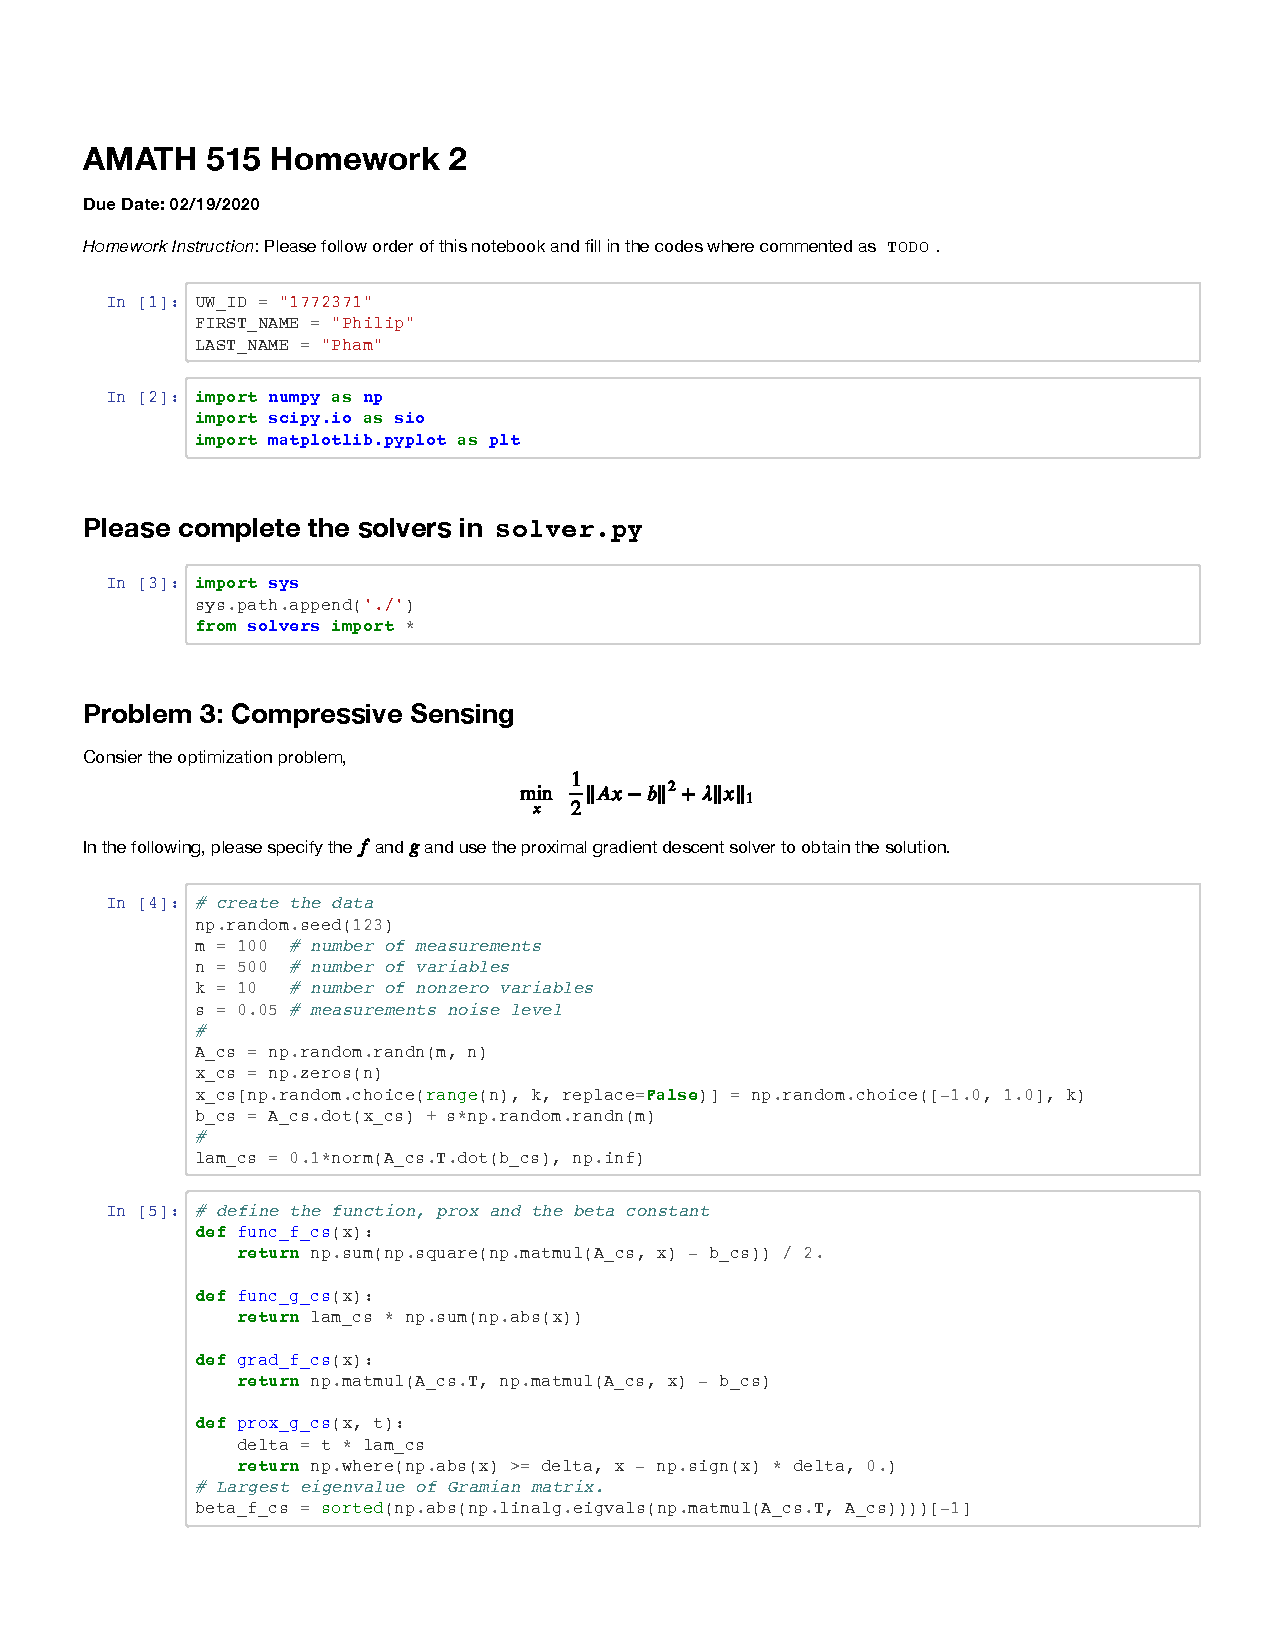
\includepdf[pages=-]{515Hw2_Coding.pdf}

\end{document}  
